\section{Algorithm}
\subsection{Continuous Equations}
2D steady-state Stokes equations for impressible flow are
\begin{equation}
    \left\{
    \begin{array}{ccc}
        -\Delta \vec u + \nabla p &=& \vec F\\
        \nabla \cdot \vec u &=&0\\
    \end{array}
    \right.
\end{equation}
where $\vec u =[u,v]^T$,$\vec F=[f,g]^T$. Sometimes, it's preferable to 
rewrite the above equations as
\begin{equation}
    \label{equ:continous}
    \left\{
    \begin{array}{ccccc}
        -\Delta u &+& \partial_x p &=& f\\
        -\Delta v &+& \partial_y p &=& g\\
        \partial_x u &+& \partial_y v &=&0\\
    \end{array}
    \right.
\end{equation}

\subsection{Finite Difference Equations}
Discretize (\ref{equ:continous}), we get
\begin{equation}
    \label{equ:discrete}
    \left\{
    \begin{array}{ccccc}
        (-\Delta)_h u_h &+& (\partial_x)_h p_h &=& f_h\\
        (-\Delta)_h v_h &+& (\partial_y)_h p_h &=& g_h\\
        (\partial_x)_h u_h &+& (\partial_y)_h v_h &=&0\\
    \end{array}
    \right.
\end{equation}
where $(\cdot)_h$ denotes the discretization on the uniform grid
whose grid size is $h$. We can rewrite (\ref{equ:discrete}) in matrix
form, so we'll see it's actually a saddle points problem.
\begin{equation}
    \label{equ:disEqu}
    \begin{bmatrix}
        A_h&B_h\\
        B_h^T&0\\
    \end{bmatrix}
    \begin{bmatrix}
        U_h\\
        p_h\\
    \end{bmatrix}
    =
    \begin{bmatrix}
        F_h\\
        0\\
    \end{bmatrix}
\end{equation}
where
\begin{equation}
    A_h=
    \begin{bmatrix}
        (-\Delta)_h&0\\
        0&(-\Delta)_h\\
    \end{bmatrix}
    \quad
    B_h=
    \begin{bmatrix}
        (\partial_x)_h\\
        (\partial_y)_h\\
    \end{bmatrix}
    \quad
    U_h=
    \begin{bmatrix}
        u_h\\
        v_h\\
    \end{bmatrix}
\end{equation}

\begin{figure}[ht]
    \centering
    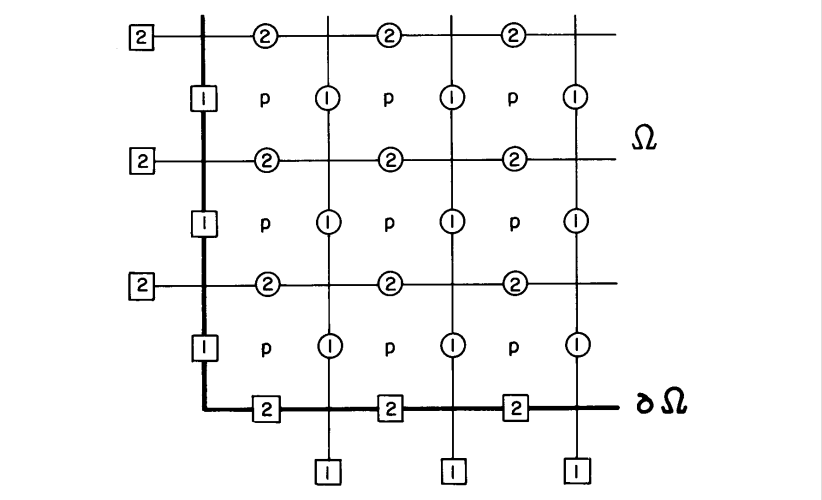
\includegraphics[width=10cm]{pic/Staggered_grid.png}
    \caption{Staggered Grid in 2D\,(\,Location 1 store $u$, Location 2 store $v$)}
\end{figure} 

Here we discretize (\ref{equ:continous}) 
on an uniform staggered grid. In 2D case, the grid define cells, and
each cell has 4 face. The discretion of x-component velocity $u$ is 
defined at the center of x-faces of cells, i.e., faces perpendicular to the 
x-coordinate. The discretion of y-component velocity $v$ is defined at the y-faces.
Discretion of pressure $p$ is located at the cell centers.

On sucn a staggered grid, we discretize the x/y-component momentum equation in x/y-face centers, 
and impressible condition $\nabla \cdot \vec u =0$ at cell centers.
Laplacian operator is approximated by five points scheme, while partial
derivative is approximated by center difference.

\subsection{Distributive Gauss-Seidal Method}
Conventional Gauss-Seidal Method  is not appliable for solving 
finite difference equation (\ref{equ:disEqu}), 
for its coefficient matrix has zero diagonal elements. So, here we use the so-called
DGS method. DGS method firstly conducts Gauss-Seidal procedure for components $u_h$ and $v_h$.
Then, for each cell,
\begin{enumerate}
    \item Compute current residual
    $$r_{ij}=F^p_{ij}-[(\partial_x)_h u_{ij}+(\partial_y)_h v_{ij}]$$
    Although here $F^p_{ij}=0$ actually, we don't omit it for the multigrid method
    \footnote{In multigrid method, we have to solve the residual equations on the 
    coarser grid, and now the right hand side on the $p$ component is not zero probably.}.
    \item Eliminate current residual
        \begin{equation}
            \begin{array}{l}
            u_{i+1/2,j}=u_{i+1/2,j}+\delta;\\
            u_{i-1/2,j}=u_{i-1/2,j}-\delta;\\
            v_{i+1/2,j}=v_{i+1/2,j}+\delta;\\
            v_{i-1/2,j}=v_{i-1/2,j}-\delta;\\
            \end{array}
        \end{equation}
        where $\delta=r_{ij}h/4$
    \item Update pressure $p$
        \begin{equation}
            \begin{array}{l}
            p_{i,j}=p_{i,j}+4\delta/h;\\
            p_{i+1,j}=p_{i+1,j}-\delta/h;\\
            p_{i-1,j}=p_{i-1,j}-\delta/h;\\
            p_{i,j+1}=p_{i,j+1}-\delta/h;\\
            p_{i,j-1}=p_{i,j-1}-\delta/h;\\
            \end{array}
        \end{equation}
        The pressure changes are in the way such that momentum-equations residuals 
        at all points remain unchange.
        If the cell is located near the boundary, the above procedure has some 
        tiny modifications. All situations are graphically presented as Figure \ref{fig:DGS}.
        \begin{figure}[ht]
            \centering
            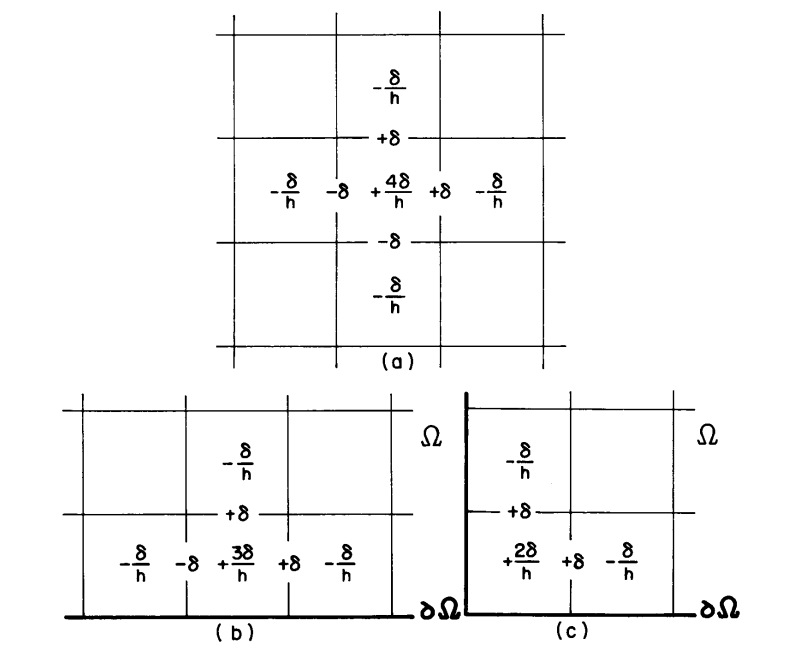
\includegraphics[width=10cm]{pic/DGS.png}
            \caption{DGS Update Cases}
            \label{fig:DGS}
        \end{figure}  
\end{enumerate}

\newpage
\subsection{Multigrid Technique}
Just as conventional Gauss-Seidal method, DGS has the same limits:
\begin{enumerate}
    \item Converge speed is slow;
    \item Converge speed declines when grid gets finer.
\end{enumerate}
Multigrid Method overcome such limits, get a much better result. See the results.